\chapter{Discussion}
\section{Water Year 2019} 
\subsection{Isothermal Snowpack and Runoff Timing}
In order to have considerable snowmelt runoff, there are three basic phases a snowpack must go through (warming, ripening, and output). Once the snowpack is isothermal, it enters the ripening phase where absorbed energy is used to melt snow. Although absorbed energy melts snow, the majority of melt water is retained in the snowpack via surface tension and continuous pores filled with air (\cite{dingman2015}). After the snowpack is nearly fully saturated with liquid water, then it is in the output phase where further absorption of energy produces water output. It is important to note that this is a very idealized sequence. For example, melting often occurs at the surface before the ripening phase and may percolate deeper into the snowpack where it can refreeze and form ice layers. In addition, latent heat exchange during these phase changes is not negligible in the overall snowpack energy balance and internal processes. 

The SNOTEL network is currently the most robust system for measuring snowpack characteristics and it creates hourly reports of snow depth, snow water equivelence (SWE), and precipitation across the Western United States. Using snow depth and SWE to calculate snow density, it is possible to estimate when a snowpack has reached ripe conditions and this is usually around 400 kg m\textsuperscript{-3} or 40\% density. The current network lacks the ability to measure snowpack temperature conditions, therefore it is very hard to predict the beginning of the ripening phase. In a scenario with a lower density snowpack at the beginning of its ripening phase, there is very little in situ measurements that provide the data necessary to make predictions on when the snowpack will enter the output phase. Combining data from the SNOTEL network, weather forecasts, and snowpack temperature arrays could provide a means to estimate the timing of the output phase. Below are fundamental equations that could be used to approach this problem. 

From empirical studies, the maximum volumetric water content ($\theta$\textsubscript{ret}) that a snowpack can retain against gravity is defined as: 
\begin{equation}
\theta \textsubscript{ret} = -0.0745\frac{\rho \textsubscript{s}}{\rho \textsubscript{w}}
+ 0.00267\frac{\rho \textsubscript{s}}{\rho \textsubscript{w}}^2 
\end{equation}
Where $\rho \textsubscript{s}$ and $\rho \textsubscript{w}$ are the densities of snow and water respectively. Ripe snowpacks usually have a bulk density of $\rho_s$ = 400 kg m\textsuperscript{-3} and according to the above equation, this leads to a maximum volumetric water content of $\theta$\textsubscript{ret} = 0.03. The net energy (Q\textsubscript{m2}) in J m\textsuperscript{-2} required to complete the ripening phase is defined as: 
\begin{equation}
Q_{m2} = \theta_{ret} * h_s * \rho_w * \lambda_f
\end{equation}
Where h\textsubscript{s} is snow depth and $\lambda_f$ is the latent heat of fusion (0.334 MJ kg\textsuperscript{-1}). 

Using weather forecasts, it is possible to estimate the potential net energy exchange between the snowpack and atmosphere. If there is a net energy exchange into the snow that exceeds Q\textsubscript{m2}, the snowpack will likely enter the output phase.  

Figures \ref{fig:0_135cm_Isothermal} - \ref{fig:0_135cm_Zoom} show snowpack temperature measurements as it reaches isothermal conditions at Banner Summit. Although the beginning of the ripening phase is defined as isothermal conditions at 0C, this study interprets isothermal conditions when the range of temperature measurements on the BSTA is minimal. The instrument's accuracy dictates this interpretation because, although it's minimal, there is an inherent error in temperature measurements. The minimum temperature range in 2019 is ~0.02 C and occurs on March 31st. This marks the beginning of the ripening phase.

The ability to precisely measure when the snowpack goes isothermal provides context when observing the following melt stages. Figure 3 shows snow density and snow water equivalence with an overlay of the interpreted melt stages. Although the snowpack goes isothermal on March 31st, the bulk density of the snowpack is still too low for any significant water output. Between the 31st - April 6th, air temperatures were below freezing, and storms brought fresh snow. During April 7th - 9th, there was rain on snow that increased snow density to ~40\%. Between April 9 - 10, the snowpack lost ~2cm of SWE, marking the beginning of the output phase.    

Using these interpretations at Banner Summit to predict runoff at the basin scale poses a few challenges.  Perhaps most significantly, to establish any relationship between these measurements and nearby streamflow, a more extended period of record is necessary. However, this dataset provides more context when interpreting springtime runoff at a nearby stream gauge. Figure \ref{fig:HydrographPhases} is a hydrograph from the nearby stream gauge with an overlay of the interpreted melt stages at Banner Summit. Shortly after the snowpack reaches the ripening phase on March 31st, streamflow at this gauge departs from normal conditions and is above the median. Additionally, when the snowpack reaches its output phase, there is a significant increase in streamflow.

\begin{figure}
    \centering
    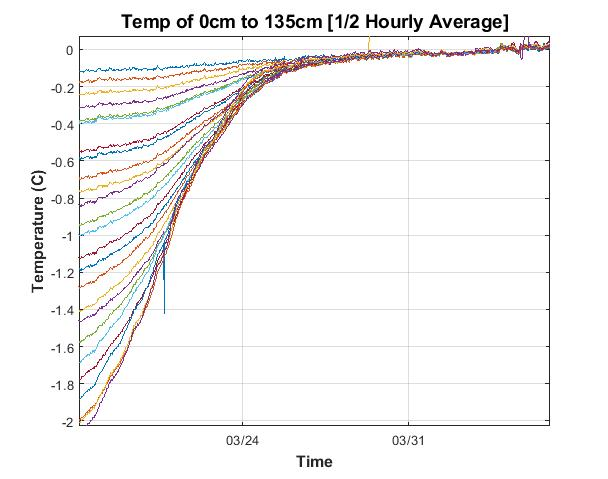
\includegraphics[width=0.7\linewidth]{figures/0_135cm_Isothermal.jpg}
    \caption{Progression of snowpack temperatures leading to isothermal conditions.}
    \label{fig:0_135cm_Isothermal}
 \end{figure}
 
 \begin{figure}
    \centering
    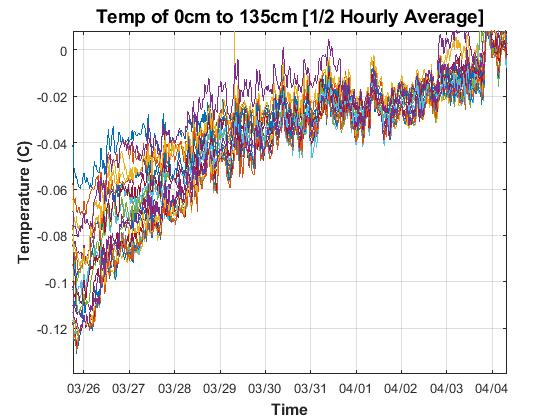
\includegraphics[width=0.7\linewidth]{figures/0_135cm_zoom.jpg}
    \caption{Sub-plot of data shown in Figure \ref{fig:0_135cm_Isothermal}}
    \label{fig:0_135cm_Zoom}
 \end{figure}
 
  \begin{figure}
    \centering
    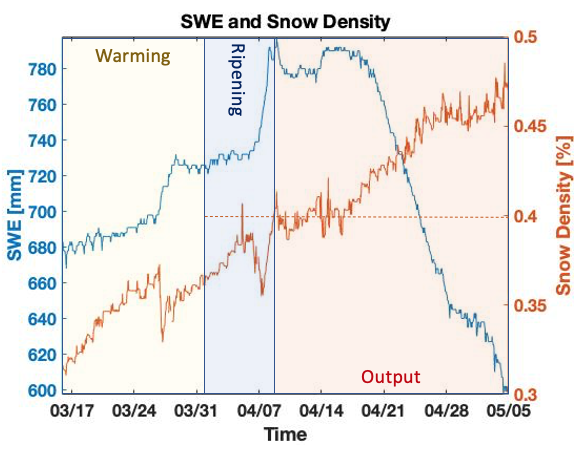
\includegraphics[width=0.8\linewidth]{figures/RunoffTiming/SWE_Density.png}
    \caption{SWE and Snow Density during the warming, ripening, and output phases at Banner Summit.}
    \label{fig:ValleyCreek}
 \end{figure}

\begin{figure}
    \centering
    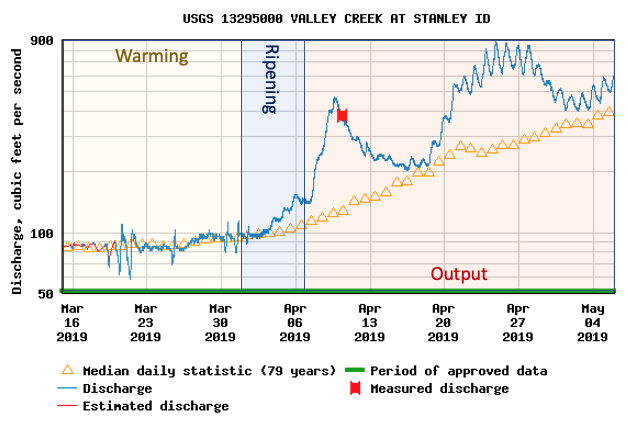
\includegraphics[width=1\linewidth]{figures/RunoffTiming/HydrographPhases.png}
    \caption{Unregulated streamflow data from a USGS stream gauge near Banner Summit.}
    \label{fig:HydrographPhases}
 \end{figure}


\subsection{Temperature Gradient Analysis}
Temperature-gradient metamorphism is the process of vapor transport along a thermal gradient (\cite{sommerfeld_1970}). As long as the gradient is maintained, as is usually the case in cold environments, the process continually acts on the snowpack. The snow characteristics during the beginning of this process have a strong effect on its progress (\cite{sommerfeld_1970}). In new, fine grained, porous snow, there are more grains in which the diffusing vapor can freeze. Resulting, the grains do not grow very large, and hollow pyramids are not common (\cite{sommerfeld_1970}). If temperature-gradient metamorphism starts in larger-grained, equi-temprature metamorphosed snow, there are fewer crystals on which the vapor can freeze. Under a consistent thermal gradient, these crystals will grow larger, and hollow pyramids along with lattice grains may be found (\cite{akitaya_1967}). 

Many different things affect the rate and nature of temperature-gradient metamorphism. Resulting, a continual collection of the snowpack temperature data is critical in understanding these processes. Further work should focus on collecting more frequent snow pit observations to document the rate of change in the snow's microstructure. 

\subsection{Stable Water Isotopes}
The 2019 isotope data have some significant random error because samples were taken in a lightly forested area with varying amounts of underbrush and fallen trees. This uneven ground creates an inconsistent datum between sampling events and introduces an unexpected amount of spatial variability. In addition to this, stable water isotopes could be effected by nearby trees and buried brush that emit longwave radiation. Moving forward, sampling for stable water isotopes in snow should be conducted in open areas with an even ground surface that is free of large brush, or fallen debris. If a study is conducted in a forested/lightly forested area, there should be a preseason effort to clear the sampling locations of anything that creates an uneven ground surface. \\

- Interpretability of WY2019 isotope dataset \\
- Future directions  \\

